\makeatletter
\@runinheadtrue
\makeatother
\cxset{style50/.style={
 name=,
 numbering=arabic,
 number font-size=LARGE,
 number font-weight=bfseries,
 number before={},
 number after=,
 number position=rightname,
 number dot=.,
 number display=block,
 number float=center,
 chapter color=black!80,
 chapter font-size=,
 chapter before=,
 number after=,
 chapter after=,
 number color=black!80,
 title font-family=rmfamily,
 title font-color=black!80,
 title before=,
 title after=\par,
 title font-weight=\bfseries,
 title font-size=\LARGE,
 title beforeskip=\space,
 title afterskip=\vspace*{20pt},
 chapter title width=0.6\textwidth,
 chapter title align=left,
 header style=empty,
 author block=true,
 author names=\textsc{\aegean James A. Russel and\\[-1.5pt] Jos\'e Miguel Fernandez-Dols },
 author block format=\normalfont\large\vskip20pt,
 epigraph width=0.8\textwidth,
 epigraph align=center,
 epigraph text align=left,
 section indent=0pt,
 section font-weight=bold,
 section align=left,
 section font-size=Large,
 subsection font-size=large,
 section number after=,}}

\cxset{style50}
\chapter{Introduction to Chapter Style Fifty: What does a facial expression mean?}
\label{ch:style50}

\epigraph{The human face -- in repose and in movement, at the moment of death as in life, in silence and in speech, when seen or seemed from within, in actuality or as recorded in art or recorded by the camera}{F. Ekman W Friesen and P. Ellsworth, 1972, p.1}

The typesetting of this book’s chapter head, although it appears simple at first it got some peculiarities and I went
back and modified some of the code to be able to handle it. As the title’s width is less than the text width it has to be typeset in a minipage. This is how normally it was done in the previous chapters, however the number was typed next to it and a kern was inserted between the number and the title. This is controlled by a switch |\@runinhead| and an equivalent key that defaults to false. 
\begin{figure}[ht]
\fbox{%
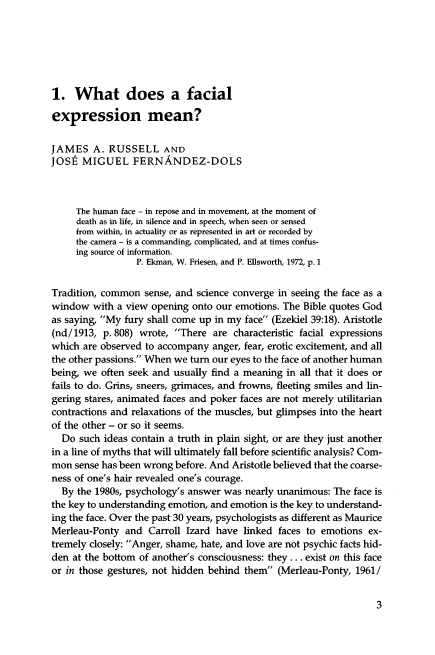
\includegraphics[width=0.48\textwidth]{./chapters/chapter50.png}\hfill
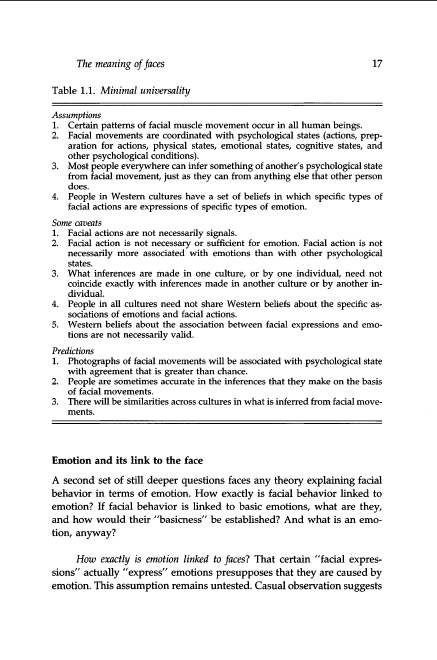
\includegraphics[width=0.48\textwidth]{./chapters/chapter50a.png}}
\caption{Style 50 from the Oxford Handbook of Cuneiform Culture.}
\label{fig:style50}
\end{figure} 
The template probably breaks all the ``rules'' of typography (such as hangindents in sections, and rules in
table heads (see Figure~\ref{fig:style50}).

\section{Loading the Template}

\begin{scriptexample}{Loading the Template}
\begin{verbatim}
\usepackage{phd}
\cxset{style50}
\end{verbatim}
\end{scriptexample}

\section{The Chapter head}
\begin{scriptexample}{Loading the Template}{}
\begin{verbatim}
\cxset{chapter format=runin}
\end{verbatim}
\end{scriptexample}

\section{Epigraph Styling}
The epigraph is similar to that of style 43 (\autoref{style43}). We are centering it, instead of just offsetting from the left margin and the epigraph text is set left:

\begin{scriptexample}{Loading the Template}
\begin{verbatim}
  epigraph width=0.8\textwidth,
  epigraph align=center,
  epigraph text align=left
\end{verbatim}
\end{scriptexample}




The psychology of facial
expression
Edited by
James A. Russell
University of British Columbia
Jose Miguel Fernandez-Dols
Universidad Autonoma de Madrid, Cambridge University Press.

\section{Images}

\begin{figure}[htbp]
\includegraphics[width=\textwidth]{facial-expression}
\caption{Image pages have running headers, something we need to set up.}
\end{figure}

\end{document}

\makeatletter\@runinheadfalse\makeatother